\section{Auswertung}
\label{sec:Auswertung}

% % Examples
% \begin{equation}
%   U(t) = a \sin(b t + c) + d
% \end{equation}
%
% \begin{align}
%   a &= \input{build/a.tex} \\
%   b &= \input{build/b.tex} \\
%   c &= \input{build/c.tex} \\
%   d &= \input{build/d.tex} .
% \end{align}
% Die Messdaten und das Ergebnis des Fits sind in Abbildung~\ref{fig:plot} geplottet.
%
% %Tabelle mit Messdaten
% \begin{table}
%   \centering
%   \caption{Messdaten.}
%   \label{tab:data}
%   \sisetup{parse-numbers=false}
%   \begin{tabular}{
% % format 1.3 bedeutet eine Stelle vorm Komma, 3 danach
%     S[table-format=1.3]
%     S[table-format=-1.2]
%     @{${}\pm{}$}
%     S[table-format=1.2]
%     @{\hspace*{3em}\hspace*{\tabcolsep}}
%     S[table-format=1.3]
%     S[table-format=-1.2]
%     @{${}\pm{}$}
%     S[table-format=1.2]
%   }
%     \toprule
%     {$t \:/\: \si{\milli\second}$} & \multicolumn{2}{c}{$U \:/\: \si{\kilo\volt}$\hspace*{3em}} &
%     {$t \:/\: \si{\milli\second}$} & \multicolumn{2}{c}{$U \:/\: \si{\kilo\volt}$} \\
%     \midrule
%     \input{build/table.tex}
%     \bottomrule
%   \end{tabular}
% \end{table}
%
% % Standard Plot
% \begin{figure}
%   \centering
%   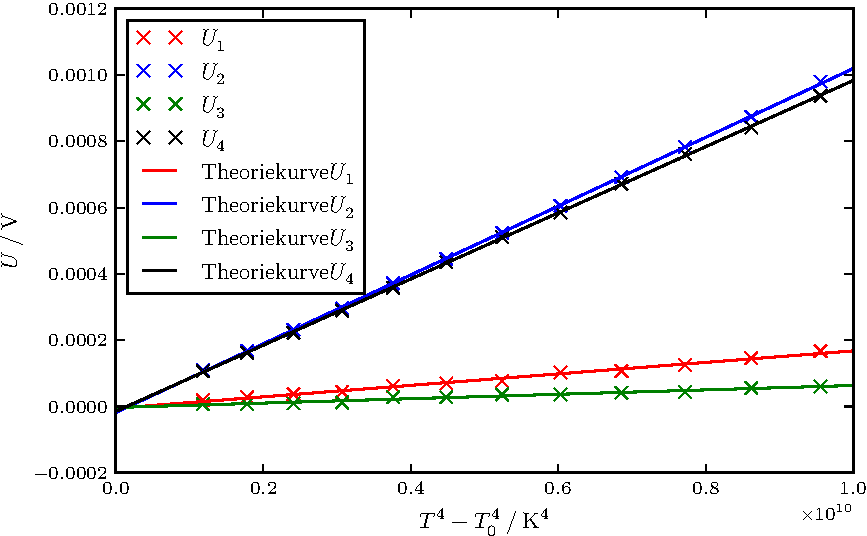
\includegraphics{build/plot.pdf}
%   \caption{Messdaten und Fitergebnis.}
%   \label{fig:plot}
% \end{figure}
%
% 2x2 Plot
% \begin{figure*}
%     \centering
%     \begin{subfigure}[b]{0.475\textwidth}
%         \centering
%         \includegraphics[width=\textwidth]{Abbildungen/Schaltung1.pdf}
%         \caption[]%
%         {{\small Schaltung 1.}}
%         \label{fig:Schaltung1}
%     \end{subfigure}
%     \hfill
%     \begin{subfigure}[b]{0.475\textwidth}
%         \centering
%         \includegraphics[width=\textwidth]{Abbildungen/Schaltung2.pdf}
%         \caption[]%
%         {{\small Schaltung 2.}}
%         \label{fig:Schaltung2}
%     \end{subfigure}
%     \vskip\baselineskip
%     \begin{subfigure}[b]{0.475\textwidth}
%         \centering
%         \includegraphics[width=\textwidth]{Abbildungen/Schaltung4.pdf}    % Zahlen vertauscht ... -.-
%         \caption[]%
%         {{\small Schaltung 3.}}
%         \label{fig:Schaltung3}
%     \end{subfigure}
%     \quad
%     \begin{subfigure}[b]{0.475\textwidth}
%         \centering
%         \includegraphics[width=\textwidth]{Abbildungen/Schaltung3.pdf}
%         \caption[]%
%         {{\small Schaltung 4.}}
%         \label{fig:Schaltung4}
%     \end{subfigure}
%     \caption[]
%     {Ersatzschaltbilder der verschiedenen Teilaufgaben.}
%     \label{fig:Schaltungen}
% \end{figure*}

\subsection{Bestimmung des Nulleffektes}
Zur Bestimmung des Nulleffektes werden zwei Messungen über einen Messbereich von $t = \SI{900}{\second}$ durchgeführt.
Es ergeben sich für zwei Messungen die Werte
\begin{align*}
  N_1 &= \num{210} \\
  N_2 &= \num{191}
\end{align*}
so dass sich ein gemittelter Nulleffekt von
\begin{align}
  \bar{N_0}&= \input{build/nulleffekt.tex}
  \label{eqn:nulleffekt}
\end{align}
ergibt.

\subsection{Bestimmung der Halbwertszeit von Indium}

Zur Bestimmung der Halbwertszeit von Indium wird ein Messintervall von $\increment t = \SI{220}{\second}$ gewählt.
Zunächst wird der Nulleffekt \eqref{eqn:nulleffekt} von den Messdaten abgezogen.
Die daraus resultierenden Messdaten sind in Tabelle \ref{tabulatore} angegeben.

\input{build/tabulatore_texformat.tex}

Daraufhin werden die gemessenen Impulse in einem halblogarithmischen Diagramm gegen die Messzeit $t$ abgetragen.
Da der radioaktive Zerfall einer statistischen Poissonverteilung unterliegt, bestimmt sich der Fehler der Messwerte zu
\begin{align*}
  \sigma &= \sqrt{x}
\end{align*}
wobei $x$ die Anzahl der gemessenen Impulse beschreibt.
Dieser Fehler wird in den Fehlerbalken angegeben.\\
Nach Gleichung \eqref{eqn:totalwichtigeformel} kann aus einer linearen Ausgleichsrechnung der logarithmierten Impulse die Zerfallskonstante $\lambda$ gewonnen werden.
Der lineare Fit wird hierbei in Python mit SciPy erstellt.
Es ergeben sich die Parameter
\begin{align*}
  -\lambda = m &= \input{build/parameter_a_indium.tex}, \\
  b &= \input{build/parameter_b_indium.tex}.
\end{align*}
Aus dem Parameter $m$ ergibt sich nach Formel \eqref{eqn:halbwertszeit} eine Halbwertszeit
\begin{align*}
  T_\text{In} &= \input{build/halbzeit_indium.tex}
\end{align*}
von Indium.
Die Ergebnisse der Messwerte und des Fits sind in Abbildung \ref{fig:plot1} dargestellt.

% Standard Plot
\begin{figure}
  \centering
  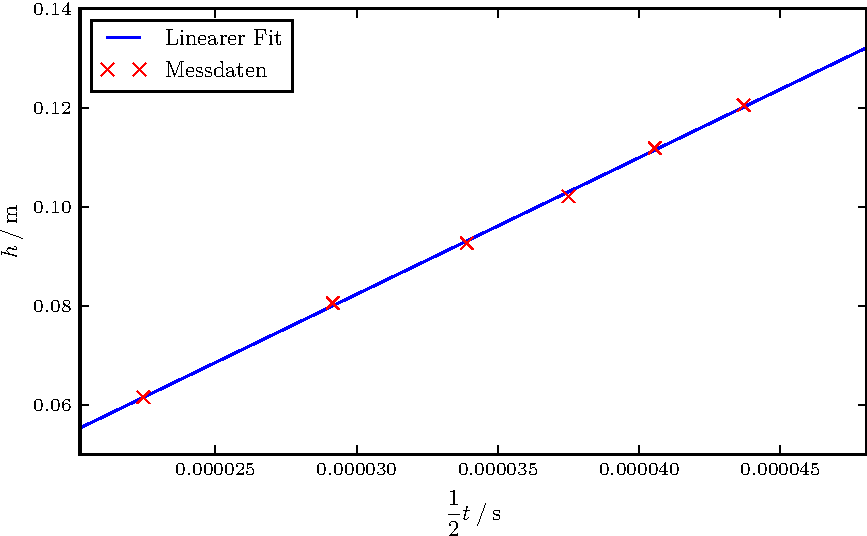
\includegraphics{build/ausgleich.pdf}
  \caption{Messdaten und linearer Fit zur Bestimmung der Halbwertszeit von Indium.}
  \label{fig:plot1}
\end{figure}

\subsection{Bestimmung der Halbwertszeit von Rhodium}

Zur Bestimmung der Halbwertszeiten von Rhodium wird ein Messintervall von $\increment t = \SI{17}{\second}$ gewählt.
Für die Messwerte wird zunächst der Nulleffekt \eqref{eqn:nulleffekt} abgezogen.
Die resultierenden Messwerte sind in Tabelle \ref{tab:2} angegeben.

%\input{build/tabulatore_texformat2.tex}

%\input{build/tabulatore_texformat3.tex}


\begin{table}
  \hspace*{\fill}
  \begin{subfigure}{0.40\textwidth}
  \centering
  %\caption{Messdaten Teil 1.}
  \label{tab:2a}
  \sisetup{table-format=3.4}
  \begin{tabular}{c c c}
    \toprule
    {$t \:/\: \si{\second}$} & {$N$} & {$N-N_0$}\\
    \midrule
    \input{build/tabulatore2.tex}
    \bottomrule
  \end{tabular}
\end{subfigure}
\hspace*{\fill}
\begin{subfigure}{0.40\textwidth}
  \centering
  %\caption{Messdaten Teil 2.}
  \label{tab:2b}
  \sisetup{table-format=3.4}
  \begin{tabular}{c c c}
    \toprule
    {$t \:/\: \si{\second}$}		& {$N$}		&
  	{$N-N_0$}		\\
    \midrule
    \input{build/tabulatore3.tex}
    \bottomrule
  \end{tabular}
\end{subfigure}
\\
\hspace*{\fill}
\hspace*{\fill}
\caption{Messdaten zur Bestimmung der Halbwertszeit von Rhodium.}
\label{tab:2}
\end{table}


Die korrigierten Messwerte werden im Diagramm \ref{fig:plot2} halblogarithmisch in rot zusammen mit dem jeweiligen Fehler gegen die Zeit $t$ aufgetragen.
\begin{figure}
  \centering
  \includegraphics{build/ausgleich2.pdf}
  \caption{Messdaten und lineare Fits zur Bestimmung der Halbwertszeiten von Rhodium.}
  \label{fig:plot2}
\end{figure}
Aufgrund der unterschiedlichen Halbwertszeiten werden zunächst die letzten 30 Messwerte betrachtet, bei denen davon ausgegangen wird, dass die Anzahl der Zerfälle des kurzlebigeren Nuklids hier vernachlässigbar klein sind.
Der lineare Fit der logarithmierten Werte nach Formel \eqref{eqn:totalwichtigeformel} ergibt somit die Parameter
\begin{align*}
  -\lambda = m &= \input{build/parameter_a_rhodium.tex}, \\
  b &= \input{build/parameter_b_rhodium.tex}.
\end{align*}
Aus dem Parameter $m$, welcher der Zerfallskonstante $\lambda$ entspricht, kann nach Formel \eqref{eqn:halbwertszeit} die Halbwertszeit von $\ce{^{104i}_45Rh }$ zu
\begin{align*}
  T_\text{Rh,1} &= \input{build/halbzeit_rhodium.tex}
\end{align*}
bestimmt werden.\\
Aus dieser ermittelten Halbwertszeit kann nun mithilfe des linearen Fits die Auswirkung auf den Zerfall des kurzlebigen Nuklids berechnet werden.
Diese korrigierten Messwerte sind in grün in Diagramm \ref{fig:plot2} mit dem jeweiligen Fehler dargestellt.
Für diese Werte wird eine weitere lineare Regression durchgeführt, welche auf die Parameter
\begin{align*}
  -\lambda = m &= \input{build/parameter_c_rhodium.tex}, \\
  b &= \input{build/parameter_d_rhodium.tex}
\end{align*}
führt.
Analog ergibt sich hieraus eine Halbwertszeit von $\ce{^{104}_45Rh }$ zu
\begin{align*}
  T_\text{Rh,2} &= \input{build/halbzeit_rhodium2.tex}.
\end{align*}
Aus beiden Zerfallskonstanten $\lambda_1$ und $\lambda_2$ kann somit eine Summenkurve berechnet werden, welche den Gesamtzerfall beschreibt.
Diese Kurve ist in Abbildung \ref{fig:plot3} angegeben.

\begin{figure}
  \centering
  \includegraphics{build/ausgleich3.pdf}
  \caption{Summenkurve aus den ermittelten Zerfallskonstanten.}
  \label{fig:plot3}
\end{figure}
